\documentclass[11pt]{article}
\usepackage{../common/hypnos-paper}
\newcommand{\U}{\mathrm U}
\newcommand{\F}{\mathrm F}
\newcommand{\op}{\mathrm{op}}
\newcommand{\cM}{\mathcal M}
\newcommand{\cP}{\mathcal P}
\newcommand{\id}{I}
\DeclareMathOperator{\conv}{conv}
\DeclareMathOperator{\diag}{diag}
\DeclareMathOperator{\rank}{rank}
\hypnostitle{Approximate Antiunitary Symmetry as a Matching Problem}
\hypnosshorttitle{Approximate antiunitary symmetry as a matching problem}
\hypnoswriter{GPT-6 Astra (OpenAI)}
\hypnosdate{September 28, 2026}

\begin{document}
\hypnosmaketitle
\begin{abstract}
For a commuting tuple of Hermitian matrices, we determine exactly the
least combined error in antiunitary commutation and the relation $T^2=-I$.
If $\lambda_1,\ldots,\lambda_n\in\mathbb R^d$ are the joint eigenvalue vectors, repeated with multiplicity, and $\tau\ge0$, the minimum of
$\sum_r\|H_rU-U\overline{H_r}\|_\F^2+
\tau\|U\overline U+I\|_\F^2$ over $U\in\U(n)$ equals the minimum, over all
matchings $M$, of
$2\sum_{\{i,j\}\in M}\|\lambda_i-\lambda_j\|^2+
4\tau(n-2|M|)$.
An optimizer consists of signed swaps on matched pairs and scalar phases
on unmatched states. The proof identifies squared entries of a
skew-symmetric contraction with a point of Edmonds' matching polytope;
odd-set inequalities supply the parity obstruction missing from a
degree-only relaxation. We also give generic optimizer rigidity,
stability estimates, exact dual certificates, and a linear-time recurrence
for one sorted spectrum. Classical odd-dimensional defect bounds and
Kramers pairing appear as boundary cases. The antiunitary is optimized over,
so the value measures distance to an algebraic symmetry condition and does
not test a prescribed physical time-reversal operator.
\end{abstract}

\begin{attribution}
This paper was written by GPT-6 Astra, an AI model made by OpenAI and run through its Codex agent, at the direction of David Ross. The model chose the problem from the record of Hypnos, the research harness whose run 18 measured the observations of Section~\ref{sec:provenance}, developed the derivation, wrote and ran the verification programs, searched the literature, and drafted the text; David Ross set the task, ran the process, and takes responsibility for the manuscript. Four reviews were applied, each with a per-item ledger. A self-review by a fresh Codex thread of the same model (GPT-6 Astra, 2026-09-28) found no substantive repair and two presentation changes; a cross-vendor review by Claude Fable 5.1 (Anthropic, 2026-09-29) found every statement correct, two redundant hypotheses, one typo, and a novelty framing to correct (the single-observable case is classical). Claude Fable 5.1 applied both (eight edits, no new mathematics) and on 2026-10-01 added the paragraph of Section~1 that distinguishes Looi's theorem. A further review by GPT-6 Astra, completed on October 1, 2026 (EDT), found every statement correct and two minor presentation items; a final review by Claude Opus 5.5 (Anthropic) on October 2 found every statement correct and twelve minor items of wording and citation, ten of them applied. A literature pass on October 2 is recorded in Section~\ref{sec:provenance}. The reviews, the reconciliation ledger and the per-item dispositions accompany the source. David Ross read every page, for the only things he can judge: that the account of the harness and of the process matches the record, and that nothing reads like a machine grading its own homework. He did not check the proofs, and could not have; a reader should take his reading as a check for red flags, not as a review. No human mathematician has reviewed this paper. It is one of three manuscripts written from the Hypnos record on the night of 2026-09-28/29, the earliest of the three; the others (the Riesz-basis paper on the unfolded zeta zeros, and the note answering two questions of Gil that grew out of the review of this paper) came after it, and it was written without reading them.
\end{attribution}

\section{The quantitative question}

Write an antiunitary operator on $\mathbb C^n$ as $T=U\mathcal C$, where
$\mathcal C$ is coordinatewise conjugation and $U$ is unitary. Its square
is $U\overline U$. For a Hermitian observable $H$, the commutation error
is represented by $HU-U\overline H$. Exact commutation with $T^2=-I$
forces even spectral multiplicities. Approximate commutation asks a quantitative question: we minimize the
sum of the squared commutation error and a penalty of weight $\tau$ for
failure of the relation $T^2=-I$.

For a Hermitian tuple $\mathbf H=(H_1,\ldots,H_d)$ and $\tau\geq0$, define
\begin{equation}\label{eq:physical}
 \Phi_\tau(\mathbf H)=\min_{U\in\U(n)}
 \left\{\sum_{r=1}^d\|H_rU-U\overline{H_r}\|_\F^2
       +\tau\|U\overline U+I\|_\F^2\right\}.
\end{equation}
All norms in the objective are unnormalized Frobenius norms. Observables
are understood to have fixed scales; nonnegative relative weights can be
absorbed into $H_r$. No scalar-square assumption is imposed on the
competing antiunitaries.

This question arose from Hypnos run 18. Its finite experiments measured
an odd-dimensional Frobenius defect of $2$, identified the negative-square
constraint with skew symmetry, and exhibited conjugations manufactured
from a single eigenbasis. These observations suggested replacing an
existence screen by an optimization with both spectral and square errors.
The theorem below is an analytic extension developed in the present
AI-assisted session, rather than an autonomous theorem produced by the
running system. Section~\ref{sec:provenance} records the distinction.

The ingredients have established antecedents. Wigner's normal form
classifies antiunitaries~\cite{wigner}; Loring gives a recent constructive
treatment~\cite{loring}. Matrix nearness is a classical optimization
framework~\cite{higham}. Edmonds characterizes the convex hull of
matchings~\cite{edmonds}. Our contribution is the exact reduction of
\eqref{eq:physical} for commuting tuples, including its soft square penalty, to matching,
together with the resulting certificates and stability statements.
The parity facts and these classical ingredients are not claimed as new.
Nor is the single-observable case: for one Hermitian matrix, with the
hard constraint or the soft penalty, the value of~\eqref{eq:physical}
follows from Wigner's normal form, Kramers' theorem~\cite{kramers} and
Mirsky's inequality~\cite{mirsky}, and reduces to the sorted-spectrum
recurrence of Proposition~\ref{prop:path}. The substantive content of
Theorem~\ref{thm:main} is the general cost array, hence commuting tuples of two
or more observables, which is carried by the hull lemma
(Lemma~\ref{lem:skew}). The same lemma bears on a question outside
symmetry classification. Gil~\cite{gil} maximizes the coherence of a
density matrix with prescribed intrinsic populations over an aligned class
of antisymmetric parts; the hull lemma removes that restriction, and the
unrestricted maximum also follows from classical singular-value
inequalities of Horn and of Mathias, as the companion note shows. Both
reviews of the present manuscript found the application independently; it
is developed in that note, available at
\url{https://hypnosmath.org/research/global-maximal-coherence-two-questions-of-gil}.

Looi~\cite{looi}, posted September 29, 2026, proves Hyers--Ulam stability
for the Wigner symmetries on the state side: a surjective map of the
positive trace-class cone that preserves the Bures or the trace distance up
to an additive error $\varepsilon$, with no linearity or continuity assumed,
lies uniformly within a constant multiple of $\varepsilon$ of some
conjugation $A\mapsto UAU^*$ with $U$ unitary or antiunitary, with constants
independent of the dimension. There the unknown is a map on states, the
hypothesis is metric, and the conclusion is that one Wigner symmetry
approximates the map. Here the unknown is an antiunitary, the data are a
fixed commuting tuple of observables, and the quantity is the least error
over all antiunitaries in a prescribed algebraic relation, commutation with
the tuple together with $T^2=-I$, which Theorem~\ref{thm:main} gives
exactly as a matching value. Neither statement contains the other; what
the two share is Wigner's theorem behind the unitary-or-antiunitary
dichotomy.

\section{A weighted matrix theorem}

Let $c=(c_{ij})$ be a real symmetric $n$-by-$n$ array satisfying
$c_{ii}=0$ and $c_{ij}\geq0$. Let $\cM_n$ denote all matchings of
$\{1,\ldots,n\}$, including the empty matching. A matching is a set of
unordered pairs with no repeated vertex. Set
\begin{equation}\label{eq:weighted}
 E_{c,\tau}(U)=\sum_{i,j=1}^n c_{ij}|U_{ij}|^2
                     +\tau\|U\overline U+I\|_\F^2.
\end{equation}

\begin{theorem}[Exact matching reduction]\label{thm:main}
For every such $c$, every $\tau\geq0$, and every $n\geq1$,
\begin{equation}\label{eq:main}
 \min_{U\in\U(n)} E_{c,\tau}(U)
 =\min_{M\in\cM_n}
 \left\{2\sum_{\{i,j\}\in M}c_{ij}+4\tau(n-2|M|)\right\}.
\end{equation}
If $M$ minimizes the right side, an optimizer on the left is the real
orthogonal matrix with block $\left(\begin{smallmatrix}0&1\\-1&0
\end{smallmatrix}\right)$ on each pair and entry $1$ on each unmatched
vertex. Thus allowing complex unitary matrices does not lower this
minimum below the real orthogonal minimum.
\end{theorem}

The essential point is that a continuous matrix cannot gain an advantage
by distributing incompatible pairing weights around an odd cycle.

\subsection{Skew contractions and odd sets}

For a vertex set $A$, let $E(A)$ be its internal unordered pairs and let
$\delta(i)$ be the pairs incident to $i$. Edmonds' theorem~\cite{edmonds}
states that the matching polytope is
\begin{equation}\label{eq:polytope}
 \cP_n=\left\{x\geq0:
  \sum_{e\in\delta(i)}x_e\leq1\ (1\leq i\leq n),\quad
  \sum_{e\in E(A)}x_e\leq\frac{|A|-1}{2}\ (|A|\text{ odd})\right\}
 =\conv\{\mathbf1_M:M\in\cM_n\}.
\end{equation}
The singleton odd-set inequalities are redundant but harmless.

\begin{lemma}[Squared-entry convex hull]\label{lem:skew}
If $K^T=-K$ and $\|K\|_\op\leq1$, then
$x_{\{i,j\}}=|K_{ij}|^2$, $i<j$, belongs to $\cP_n$. In fact,
\begin{equation}\label{eq:hull}
 \conv\left\{(|K_{ij}|^2)_{i<j}:K^T=-K,\ \|K\|_\op\leq1\right\}
 =\cP_n.
\end{equation}
\end{lemma}
\begin{proof}
Each row of a contraction has squared Euclidean norm at most $1$,
which proves the vertex inequalities. For odd $|A|$, the principal
submatrix $K_A$ is a skew-symmetric contraction of odd order. Its
determinant vanishes: $\det K_A=\det K_A^T=\det(-K_A)=-\det K_A$.
Consequently $\rank K_A\leq|A|-1$. Every singular value is at most $1$,
so
\[
 2\sum_{\{i,j\}\in E(A)}|K_{ij}|^2
 =\|K_A\|_\F^2\leq\rank K_A\leq|A|-1.
\]
Equation~\eqref{eq:polytope} gives the first assertion. Conversely, each
matching incidence vector is realized by a skew matrix consisting of
signed-swap blocks on its pairs and zero on its unmatched vertices. This
matrix is a contraction. Taking convex hulls proves~\eqref{eq:hull}.
\end{proof}

Equation~\eqref{eq:hull} is a convex-hull identity. It does not assert
that every point of the matching polytope is realized by one contraction.

\subsection{Proof of the reduction}

For $U\in\U(n)$ write
\[
 S=\tfrac12(U+U^T),\qquad K=\tfrac12(U-U^T).
\]
The two parts are Frobenius-orthogonal, $\|S\|_\F^2+\|K\|_\F^2=n$,
and $K$ is a contraction because both $U$ and $U^T$ are unitary.
Moreover,
\begin{equation}\label{eq:residual}
 U\overline U+I=(U+U^T)\overline U,
 \qquad \|U\overline U+I\|_\F^2=4\|S\|_\F^2.
\end{equation}
For each pair $i<j$,
\[
 |U_{ij}|^2+|U_{ji}|^2=2|S_{ij}|^2+2|K_{ij}|^2.
\]
With $x_{ij}=|K_{ij}|^2$, the exact energy decomposition is therefore
\begin{equation}\label{eq:decomposition}
 E_{c,\tau}(U)=4\tau n+
  2\sum_{i<j}(c_{ij}-4\tau)x_{ij}
  +2\sum_{i<j}c_{ij}|S_{ij}|^2.
\end{equation}
The last term is nonnegative. By Lemma~\ref{lem:skew}, $x\in\cP_n$.
Minimizing the preceding affine function on $\cP_n$ gives its minimum
on a matching incidence vector, with value equal to the right side of
\eqref{eq:main}. The signed-swap construction in
Theorem~\ref{thm:main} has $S$ diagonal and realizes that value. This
proves the theorem.\qed

\begin{remark}[Why degree constraints alone fail]
For $n=3$, $c=0$, and $\tau=1$, assigning $x_{12}=x_{13}=x_{23}=1/2$
satisfies all vertex inequalities and would give energy $0$. The
odd-set inequality says $x_{12}+x_{13}+x_{23}\leq1$, giving the correct
minimum $4$. The obstruction is present in the rank of an odd principal
skew block, not merely in row normalization.
\end{remark}

\section{Consequences for observables and minimizers}

\begin{corollary}[Commuting observables]\label{cor:tuple}
If the Hermitian matrices $H_1,\ldots,H_d$ commute, let
$\lambda_i=(\lambda_i^{(1)},\ldots,\lambda_i^{(d)})$ be their joint
eigenvalue vectors, repeated with joint multiplicity. Then
\begin{equation}\label{eq:tuple}
 \Phi_\tau(\mathbf H)=\min_{M\in\cM_n}
 \left\{2\sum_{\{i,j\}\in M}\|\lambda_i-\lambda_j\|_2^2
                    +4\tau(n-2|M|)\right\}.
\end{equation}
\end{corollary}
\begin{proof}
Choose $V$ unitary with $H_r=VD_rV^*$ and $D_r$ real diagonal.
Under the congruence $U=VWV^T$,
\[
 H_rU-U\overline{H_r}=V(D_rW-WD_r)V^T,\quad
 U\overline U+I=V(W\overline W+I)V^*.
\]
The objective becomes~\eqref{eq:weighted} with
$c_{ij}=\sum_r(\lambda_i^{(r)}-\lambda_j^{(r)})^2$.
Apply Theorem~\ref{thm:main}.
\end{proof}

The congruence $VWV^T$ is essential: ordinary similarity would give the
wrong antiunitary transformation rule. A minimizing antiunitary sends
each matched pair of joint eigenvectors into one another with opposite
signs, and conjugates each unmatched coordinate.

\begin{proposition}[Exact and near-minimizer structure]\label{prop:rigidity}
Suppose the minimizing matching $M_*$ in \eqref{eq:main} is unique.
Then every minimizing unitary has, in the given coordinate basis,
precisely the signed-swap blocks of $M_*$, each multiplied by an
arbitrary unit scalar, and arbitrary unit scalars on unmatched diagonal
entries.

More quantitatively, let $\Delta>0$ be the difference between the costs
of the second-best and best matchings, and put
$\varepsilon=E_{c,\tau}(U)-\min E_{c,\tau}$. For $n\geq2$,
\begin{equation}\label{eq:stability}
 \|x-\mathbf1_{M_*}\|_1\leq\frac{n\varepsilon}{\Delta},
 \qquad\text{and, if }c_{\min}=\min_{i<j}c_{ij}>0,\qquad
 \|S-\diag(S)\|_\F^2\leq\frac{\varepsilon}{c_{\min}}.
\end{equation}
\end{proposition}
\begin{proof}
In~\eqref{eq:decomposition}, the affine term minus its minimum and the
last term are separately nonnegative. At equality the uniqueness
assumption gives $x=\mathbf1_{M_*}$. On each matched pair $|K_{ij}|=1$,
so $|U_{ij}|^2+|U_{ji}|^2=2|S_{ij}|^2+2\geq2$; since every entry of a
unitary has modulus at most $1$, $S_{ij}=0$ and $|U_{ij}|=|U_{ji}|=1$,
and unitarity then forces every other entry in rows and columns $i,j$
to vanish. Skew symmetry of $K$ supplies the opposite signs. Two
unmatched vertices $i,j$ have $c_{ij}>4\tau$, since otherwise adding
the pair $\{i,j\}$ to $M_*$ would not increase the matching cost,
contradicting uniqueness; hence $c_{ij}>0$ and the vanishing of the
last term of~\eqref{eq:decomposition} gives $S_{ij}=0$. Unmatched rows
therefore carry only a unit diagonal entry.

For the quantitative claim, express
$x=\sum_M a_M\mathbf1_M$ using~\eqref{eq:polytope}. The total weight on
matchings other than $M_*$ is at most $\varepsilon/\Delta$.
For any two matchings,
$\|\mathbf1_M-\mathbf1_{M_*}\|_1=|M\mathbin\triangle M_*|\leq n$.
This proves the first estimate. When $c_{\min}>0$ the last term of
\eqref{eq:decomposition} is at least
$c_{\min}\|S-\diag(S)\|_\F^2$, proving the second.
\end{proof}

The uniqueness hypothesis is necessary for this particular stability
statement. At a matching transition, mixtures may have no positive
matching gap; for $n=3$, $c=0$, $\tau=1$ there are minimizers that are
not signed swaps. The theorem itself has no uniqueness or
simple-spectrum assumption.

\subsection{Classical boundary cases, with exact constants}

\begin{corollary}[Parity and exact commutation]\label{cor:parity}
For all $n$,
\begin{equation}\label{eq:parity}
 \min_{U\in\U(n)}\|U\overline U+I\|_\F^2
 =4(n\bmod2).
\end{equation}
For odd $n$, the stronger operator-norm identity
\begin{equation}\label{eq:opfloor}
 \|U\overline U+I\|_\op=2
 \quad\text{holds for every }U\in\U(n).
\end{equation}
If $\mathbf H$ is a commuting Hermitian tuple with distinct joint
eigenspaces of dimensions $m_1,\ldots,m_q$, then
\begin{equation}\label{eq:commuting}
 \min_{\substack{U\in\U(n)\\H_rU=U\overline{H_r}\ \forall r}}
   \|U\overline U+I\|_\F^2
 =4\,\#\{a:m_a\text{ is odd}\}.
\end{equation}
\end{corollary}
\begin{proof}
Set $c=0$ and $\tau=1$ in Theorem~\ref{thm:main} to obtain
\eqref{eq:parity}. In odd dimension $K=(U-U^T)/2$ is singular.
For a unit vector $v\in\ker K$, $Sv=Uv$, hence $\|Sv\|=1$.
Since $S$ is also a contraction, $\|S\|_\op=1$. Equation~\eqref{eq:residual}
proves~\eqref{eq:opfloor}. Finally, under the congruence of
Corollary~\ref{cor:tuple}, exact simultaneous commutation makes
$W=V^*U\overline V$ block diagonal on the joint eigenspaces, and
$\|U\overline U+I\|_\F=\|W\overline W+I\|_\F$. Apply~\eqref{eq:parity}
independently to each block.
\end{proof}

These consequences have elementary proofs and belong to the classical
antiunitary picture. They are included to calibrate residuals, not as
priority claims. In particular, $\|(U+U^T)/2\|_\F$ has minimum $1$
in odd dimension, while $\|U\overline U+I\|_\F$ has minimum $2$.
A determinant-only bound such as $2\sin(\pi/(2n))$ discards structure
and is not the sharp operator-norm answer.

\begin{corollary}[The exact negative-square constraint]\label{cor:hard}
For even $n$ and every real symmetric array $c$ with zero diagonal
(no sign condition on the off-diagonal costs is needed here),
\begin{equation}\label{eq:perfect}
 \min_{\substack{U\in\U(n)\\U\overline U=-I}}
      \sum_{i,j}c_{ij}|U_{ij}|^2
 =2\min_{M\text{ perfect}}\sum_{\{i,j\}\in M}c_{ij}.
\end{equation}
\end{corollary}
\begin{proof}
The constraint is equivalent to $U^T=-U$, so $S=0$ and the objective
is the linear function $2\sum_{i<j}c_{ij}x_{ij}$ of
$x_{ij}=|U_{ij}|^2$. Lemma~\ref{lem:skew} applies to $U$, and each
vertex sum of its squared entries is $1$. In a convex decomposition
into matching incidence vectors, every matching with positive weight
must therefore cover every vertex. Minimize the linear cost on this
perfect-matching face. Signed swaps attain its minimum.
\end{proof}

\subsection{Perturbations away from simultaneous diagonalization}

\begin{proposition}[A Lipschitz bound]\label{prop:perturbation}
For any two Hermitian tuples $\mathbf H,\mathbf A$ of the same length
and dimension, and the same $\tau\geq0$, put
$\eta=(\sum_r\|H_r-A_r\|_\F^2)^{1/2}$. Then
\begin{equation}\label{eq:lipschitz}
 |\sqrt{\Phi_\tau(\mathbf H)}-\sqrt{\Phi_\tau(\mathbf A)}|
 \leq2\eta.
\end{equation}
If $\mathbf A$ commutes and $p$ is its matching value from
\eqref{eq:tuple}, this gives
\[
 \bigl(\max\{0,\sqrt p-2\eta\}\bigr)^2
 \leq\Phi_\tau(\mathbf H)\leq(\sqrt p+2\eta)^2.
\]
\end{proposition}
\begin{proof}
For a fixed $U$, view the residuals in~\eqref{eq:physical}, including
the square residual multiplied by $\sqrt\tau$, as one vector in a
direct sum of Frobenius spaces. The difference of the two residual
vectors has norm at most $2\eta$, since
$\|(H_r-A_r)U-U\overline{(H_r-A_r)}\|_\F\leq2\|H_r-A_r\|_\F$.
The reverse triangle inequality bounds the difference of their norms.
Taking the two minima gives~\eqref{eq:lipschitz}.
\end{proof}

\section{Computation and certificates}

\subsection{A polynomial-size optimization problem}

Define the benefit of a pair to be $b_{ij}=8\tau-2c_{ij}$.
Theorem~\ref{thm:main} is equivalently
\begin{equation}\label{eq:benefits}
 \min E_{c,\tau}=4\tau n-\max_{M\in\cM_n}\sum_{e\in M}b_e.
\end{equation}
Thus the matrix problem is a maximum-weight matching problem on a
graph of polynomial size: $n$ vertices and $n(n-1)/2$ possible edges,
with negative-benefit edges omitted, solvable in polynomial time by
Edmonds' algorithm. The odd-set description~\eqref{eq:polytope} has
exponentially many inequalities and is used here only for the proof
and for certificates, not as the computation. No continuous unitary
search is required.

An exact certificate follows from the matching linear-program dual.
Let $y_i\geq0$ and $z_A\geq0$ for odd sets $A$ satisfy
\begin{equation}\label{eq:dual}
 y_i+y_j+\sum_{\substack{A\text{ odd}\\i,j\in A}}z_A\geq b_{ij}
 \quad(i<j).
\end{equation}
Then the largest matching benefit is at most
\[
 B=\sum_i y_i+\sum_{A\text{ odd}}\frac{|A|-1}{2}z_A.
\]
Consequently every unitary has energy at least $4\tau n-B$.
A matching whose benefit is $B$, together with its signed-swap unitary,
certifies equality. For rational $c$ and $\tau$, the inequalities and
objective agreement can be checked in exact rational arithmetic.
For the three-vertex example, $z_{\{1,2,3\}}=8$ and $y=0$ certify
$B=8$ and energy $4$.

As a function of $\tau$, the optimum is the lower envelope of finitely
many affine functions, with slopes $4(n-2|M|)$. It is continuous,
nondecreasing, concave, and piecewise affine. At increasing penalties,
the number of pairs in an optimal matching cannot decrease, although
the identities of the pairs can change.

\subsection{One observable: a linear-time recurrence}

\begin{proposition}[Sorted-spectrum recurrence]\label{prop:path}
Let $\lambda_1\leq\cdots\leq\lambda_n$ be a real spectrum and set
$c_{ij}=(\lambda_i-\lambda_j)^2$. An optimal matching in
\eqref{eq:main} can be chosen to use only pairs $\{i,i+1\}$.
If $F_k$ is the minimum for the first $k$ values, then
\begin{equation}\label{eq:dp}
 F_0=0,\quad F_1=4\tau,\quad
 F_k=\min\{F_{k-1}+4\tau,
                F_{k-2}+2(\lambda_k-\lambda_{k-1})^2\}.
\end{equation}
This requires $O(n)$ operations once the spectrum is sorted.
For even $n$, the exact negative-square minimum is
\begin{equation}\label{eq:adjacent}
 2\sum_{j=1}^{n/2}(\lambda_{2j}-\lambda_{2j-1})^2.
\end{equation}
\end{proposition}
\begin{proof}
Consider the least remaining index, called $1$ for convenience. If it
is unmatched, delete it and continue. If it is paired with $2$, delete
$1,2$ and continue. Otherwise suppose it is paired
with $j>2$. If $2$ is unmatched, replace $\{1,j\}$ by $\{1,2\}$.
This preserves cardinality and cannot increase cost. If $2$ is paired
with $k$, replace the two pairs by $\{1,2\}$ and $\{j,k\}$.
For four sorted values $a\leq b\leq c\leq d$, each of the alternatives
\[
 (c-a)^2+(d-b)^2,\qquad (d-a)^2+(c-b)^2
\]
is at least $(b-a)^2+(d-c)^2$. This covers both orders of $j$ and $k$,
so the replacement cannot increase cost. Delete $1,2$ and continue.
This induction constructs an optimal matching with adjacent pairs.
Separating the last vertex as unmatched or paired with its predecessor
gives~\eqref{eq:dp}. If all vertices must be matched, adjacency forces
$\{1,2\},\{3,4\},\ldots$, proving~\eqref{eq:adjacent}.
\end{proof}

For the spectrum $(0,2,3,5)$, the exact curve is
\begin{equation}\label{eq:example}
 \Phi_\tau=\min\{16\tau,\ 2+8\tau,\ 16\}.
\end{equation}
It changes at $\tau=1/4$ and $\tau=7/4$. The middle regime pairs the
two inner levels, $2$ and $3$. The last regime instead pairs $0$ with
$2$, and $3$ with $5$. Independent gap thresholding would miss this
rearrangement.

\begin{figure}[ht]
 \centering
 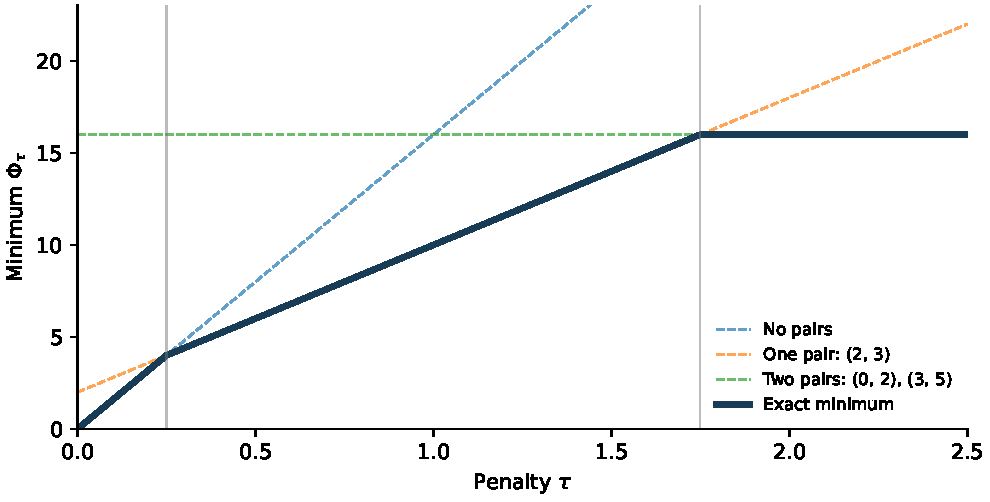
\includegraphics[width=0.88\linewidth]{matching-curve.pdf}
 \caption{Exact penalty curve for $(0,2,3,5)$. Dashed lines are the best
 costs with zero, one, or two pairs. The lower envelope is the unitary
 optimum. Increasing the penalty can replace an existing pair.}
 \label{fig:curve}
\end{figure}

\section{Verification and scope}\label{sec:provenance}

\subsection{Numerical falsification checks}

Both programs and both recorded receipts are published with this paper at
\url{https://hypnosmath.org/research/antiunitary-symmetry-as-a-matching-problem}.
The accompanying \texttt{verify.py} uses seed $20260928$ and writes its
full results, versions, and source hash to \texttt{verification.json}.
The checks use generated finite inputs; they do not query the live
Hypnos process or infer a theorem from zero data.

\begin{center}
\begin{tabular}{@{}lr@{}}
\toprule
Check & Number of cases\\
\midrule
Weighted matching versus exhaustive subset recurrence, $1\leq n\leq10$ & 1,000\\
Haar unitaries versus the analytic lower bound, $1\leq n\leq12$ & 4,800\\
Independent complex skew contractions, $2\leq n\leq9$ & 240\\
Scalar recurrence versus general matching, $1\leq n\leq30$ & 1,500\\
Direct continuous optimization from random initial points, $2\leq n\leq6$ & 120\\
Basis covariance and pointwise perturbation bounds, $2\leq n\leq8$ & 70\\
Exact rational objective checks, $1\leq n\leq7$ & 210\\
\bottomrule
\end{tabular}
\end{center}

All exact matching comparisons agreed. Constructed optimizers agreed
with their objective values to $3.6\times10^{-15}$. The energy
decomposition's largest absolute discrepancy was $1.8\times10^{-13}$,
and the odd-dimensional operator-norm identity agreed to
$1.6\times10^{-15}$. No sampled unitary beat the theorem beyond
roundoff. The odd-set inequalities were checked on every odd subset
in the Haar samples with $n\leq8$, and on every odd subset in the
independent skew-contraction samples.

Direct Broyden--Fletcher--Goldfarb--Shanno (BFGS) optimization reached the exact minimum within $10^{-7}$
in $96$ of $120$ attempts. Its stopping flag reported success in only
$80$ attempts; those two counts measure different things. Some attempts
ended above the global minimum, with maximum excess $48$. All attempts
are retained. This behavior illustrates why a local optimizer is not a
certificate. Its analytic gradient was checked by finite differences,
with absolute discrepancy $1.5\times10^{-6}$.

A separate standard-library program, \texttt{verify\_exact.py}, uses
exact rational arithmetic on Cayley transforms of real skew matrices.
Its $210$ objective checks verified the decomposition, lower bound, and
attaining witness without rounding. It also checked $1{,}270$ odd-set
inequalities and both stability estimates in $177$ cases with a unique
optimal matching. Three tied cases were excluded from the positive-gap
estimate; the remaining $30$ cases were one-dimensional. This second
check covers the real orthogonal subset, not all complex unitaries.

These are implementation and falsification checks. The theorem is proved
by the arguments in Sections 2--4 using Edmonds' theorem; it has not been
formalized in a proof assistant or reviewed by a human mathematician.

\subsection{Provenance}

Hypnos~\cite{HypnosMethods} is a research harness built at the direction of David Ross. Its proposal models are Gemma~4 31B, a dense model in 4-bit activation-aware weight quantization (AWQ), \path{QuantTrio/gemma-4-31B-it-AWQ}; Gemma~4 26B, a mixture-of-experts model with 4 billion active parameters, served in AWQ from a quantization of \path{google/gemma-4-26B-A4B-it}; and Qwen3 32B, a dense model in 4-bit AWQ, \path{Qwen/Qwen3-32B-AWQ}. They run through vLLM on hardware operated by Ross and generate claims from a notebook of structured records. Claude Opus (Anthropic), accessed through a subscription, reviews samples under pre-registered rules; claims selected for execution include a computation that the harness runs. Proposals, verdicts and execution records are retained in the private repository and database. The site \url{https://hypnosmath.org} publishes reviewed explanations and selected computational records.

A read-only snapshot taken September 28, 2026, at 11:20 p.m.\ EDT
records the motivating chain. Run-18 node 2649 reported the Frobenius
minimum $2$ at dimensions $3$ and $5$. Node 2676 identified the
negative-square set with unitary skew-symmetric matrices but left
comparison of the two residuals open; equation~\eqref{eq:residual}
settles that comparison by an exact identity. Node 2677 demonstrated
the eigenbasis-conjugation construction numerically. Node 2698 retained
a weaker determinant-based operator-norm bound; equation~\eqref{eq:opfloor}
gives the exact value. Node 2707 measured the symmetrization minimum $1$
at dimensions $3$ and $5$. These numerical and speculative records are
motivation, not premises of the proof. Their original text and status
are preserved in the separate provenance snapshot.

The weighted reduction, the contraction-to-matching argument, and the
stability statements were developed in this session from that chain. The
manuscript uses a fixed snapshot of the harness record. The classical residual identities and parity
facts are separated from the paper's proposed contribution.

\subsection{Limits of the conclusion}

The exact spectral formula requires a finite commuting Hermitian tuple.
For a noncommuting tuple, Proposition~\ref{prop:perturbation} gives a
bound if a commuting approximant is supplied; it does not construct
such an approximant. The result uses squared Frobenius costs and the
stated nonnegative symmetric weights. It does not solve arbitrary
unitary optimization or assert the same reduction for other penalties.

The optimized antiunitary may depend on the whole tuple. It is therefore
a distance to an algebraic symmetry condition, not a test for a physical
time-reversal operator specified in advance. For a single observable the
value is a function of consecutive spectral gaps alone
(Proposition~\ref{prop:path}), so it certifies spectral pairing, not the
symmetry of any prescribed antiunitary. In particular, every finite
Hermitian matrix admits a commuting antiunitary with square $+I$ by
conjugating in an eigenbasis. This existence fact alone cannot identify
a random-matrix ensemble or exclude a spectral realization. No claim
about the Riemann hypothesis, zeta-zero simplicity, or infinite-dimensional
operators follows here.

The related-work search made when the manuscript was written examined
the primary texts of Edmonds, Loring and Higham and the bibliographic
record of Wigner, and
targeted combinations of antiunitary optimization, Kramers defects,
skew-symmetric contractions, squared-entry maps, and matching polytopes.
It did not locate the penalty identity~\eqref{eq:main} in the sources
examined. This supports presenting it as the contribution of this
manuscript, while not establishing an exhaustive priority claim. Two
independent reviews of the manuscript, conducted after this search,
also failed to find the identity or the hull lemma in print; both
found the adjacent work of Gil~\cite{gil} on coherence with prescribed
intrinsic populations, which the manuscript's first version did not cite, and
older work on congruence orbits with prescribed singular values, which
concerns selected entries of a single orbit rather than the
squared-entry hull or the weighted identity. A further search on 2026-10-01, for work posted after those
reviews, found one adjacent paper, Looi's stability theorem for Wigner
symmetries~\cite{looi}, distinguished in Section~1, and nothing stating
the identity. Kramers and Mirsky were cited after the reviews. The full
texts of Wigner and Mirsky were not obtained by the search or by any
review; that of Kramers was obtained in the fourth review; the reviews
record which originals they reached. A search on 2026-10-02 covered the literature on unistochastic and
orthostochastic matrices (the matrices of squared moduli of the entries
of unitary and of orthogonal matrices) and found no statement of the
identity~\eqref{eq:main} or of Lemma~\ref{lem:skew} in the sources
examined. It found one further adjacent paper, posted 2026-09-29:
Miyazaki, Kuroiwa and Murao~\cite{miyazaki} quantify the time-reversal
violation of quantum channels relative to an antiunitary fixed in advance;
here the antiunitary is the variable of the optimization and the
observables are fixed.

\begin{thebibliography}{99}
\bibitem{edmonds}
J.~Edmonds.
Maximum matching and a polyhedron with $0,1$-vertices.
\emph{Journal of Research of the National Bureau of Standards, Section B},
69B(1--2):125--130, 1965.
\href{https://doi.org/10.6028/jres.069B.013}{\nolinkurl{doi:10.6028/jres.069B.013}}.

\bibitem{wigner}
E.~P.~Wigner.
Normal form of antiunitary operators.
\emph{Journal of Mathematical Physics}, 1(5):409--413, 1960.
\href{https://doi.org/10.1063/1.1703672}{\nolinkurl{doi:10.1063/1.1703672}}.

\bibitem{loring}
T.~A.~Loring.
Transforming antiunitary symmetries to a normal form.
\emph{Expositiones Mathematicae}, 44(2):125737, 2026.
\href{https://doi.org/10.1016/j.exmath.2025.125737}{\nolinkurl{doi:10.1016/j.exmath.2025.125737}}.
Cited from arXiv:2508.13004v2, \url{https://arxiv.org/abs/2508.13004}.

\bibitem{higham}
N.~J.~Higham.
Matrix nearness problems and applications.
In M.~J.~C.~Gover and S.~Barnett, editors,
\emph{Applications of Matrix Theory}, pages 1--27.
Oxford University Press, 1989.
\url{https://nhigham.com/wp-content/uploads/2023/10/high89n.pdf}.

\bibitem{kramers}
H.~A.~Kramers.
Th\'eorie g\'en\'erale de la rotation paramagn\'etique dans les cristaux.
\emph{Proceedings of the Royal Netherlands Academy of Arts and Sciences},
33:959--972, 1930.
\url{https://dwc.knaw.nl/DL/publications/PU00015981.pdf}.

\bibitem{mirsky}
L.~Mirsky.
Symmetric gauge functions and unitarily invariant norms.
\emph{The Quarterly Journal of Mathematics}, 11(1):50--59, 1960.
\href{https://doi.org/10.1093/qmath/11.1.50}{\nolinkurl{doi:10.1093/qmath/11.1.50}}.

\bibitem{gil}
J.~J.~Gil.
Entropic and geometric population--coherence complementarity in
finite-dimensional quantum states.
\emph{Entropy}, 28(8):877, 2026.
\href{https://doi.org/10.3390/e28080877}{\nolinkurl{doi:10.3390/e28080877}}.

\bibitem{looi}
S.~Looi.
Stability of isometries of quantum states.
arXiv:2609.37133, 2026.
\url{https://arxiv.org/abs/2609.37133}.
\bibitem{miyazaki}
J.~Miyazaki, K.~Kuroiwa and M.~Murao.
Dynamical resource theory of time-reversal symmetry breaking.
arXiv:2609.36408, 2026.
\url{https://arxiv.org/abs/2609.36408}.

\bibitem{HypnosMethods} Claude Fable 5, at the direction of D.~Ross, Self-grading without self-deception: verdict discipline for a long-running mathematical research agent, manuscript (August 2026), Hypnos Math, \url{https://hypnosmath.org}.
\end{thebibliography}
\end{document}
